%% =========================================================
%%  ProTrader AI — IJCDS Research Paper (Revised, RO-aligned)
%% =========================================================

\myabstract[1]{%
\vspace{-1cm}\hrule\vspace{2mm}
\textbf{Abstract:}
Equity price forecasting in emerging markets such as India is complicated by
multilingual news flows, regime changes, structural illiquidity, and a
heterogeneous mix of retail and institutional participants.
We present \emph{ProTrader AI}, a hybrid ensemble with an open-source
implementation that fuses four data streams---Open-High-Low-Close-Volume (OHLCV) time series,
multi-source news and social-media sentiment scored by a domain-adapted FinBERT
model with multilingual support, Foreign and Domestic Institutional Investor
(FII/DII) flows, and macroeconomic state variables---into a Ridge-stacked
classifier and a conformal quantile regressor.
The system is explicitly designed around four research objectives: (RO1)
comprehensive multi-source data integration; (RO2) a hybrid large-language-model
(LLM) plus indicator framework for real-time prediction; (RO3) an explainable
AI layer with temporal sentiment-to-price dynamics analysis; and (RO4)
cross-market transfer learning evaluation.
On a 2024 holdout of NIFTY~50 constituents, ProTrader~AI achieves
\textbf{59.3\%} directional accuracy (95\% block-bootstrap CI [56.1\%, 62.7\%];
block length~5, reflecting cross-sectional dependence across 50 tickers),
Expected Calibration Error (ECE) of \textbf{4.2\%}, Brier score \textbf{0.218},
and Sharpe ratio \textbf{1.34}, with a Diebold--Mariano $p\!=\!0.031$ against
buy-and-hold. XGBoost-component SHAP attribution identifies FinBERT sentiment as
the single most influential feature (mean absolute SHAP value
$\bar{|\phi|}\!=\!0.182$), and Granger-causality testing reveals a significant
one-day sentiment lead ($p\!=\!0.018$). A zero-shot
cross-market transfer to an S\&P~500 subset yields 55.8\% accuracy, rising to
57.6\% after a lightweight 30-day fine-tune of the stacking layer only.
\newline\newline
\textbf{Keywords:} stock market prediction; multi-source data fusion; FinBERT;
ensemble learning; conformal prediction; SHAP; transfer learning; Indian equity
markets; explainable AI.
\vspace{1mm}\hrule}

\maketitle

%% =========================================================
\section{INTRODUCTION}
\label{sec:intro}
%% =========================================================

\setlength{\parindent}{5mm}

The application of artificial intelligence to financial decision-making has
accelerated dramatically, driven by the availability of high-frequency market
data, alternative data streams, and large pre-trained language models~\cite{rahmani2023ai}.
Yet, despite measurable progress, three persistent gaps remain: (i)~most
published systems fuse at most two data modalities, ignoring the complementary
signal carried by macroeconomic state and institutional order-flow; (ii)~probabilistic
outputs are rarely calibrated, making the resulting confidence scores unsafe for
risk-proportional position sizing; and (iii)~very few studies validate
cross-market generalisation, leaving open whether a model trained on one exchange
transfers to another.

The Indian National Stock Exchange (NSE) presents a particularly demanding
testbed. It hosts approximately 2{,}000 actively traded equities and combines
foreign institutional investors (FIIs), domestic institutions (DIIs), and a
rapidly expanding retail base whose decisions are shaped by news-app feeds in
both English and Hindi. Nti~\etal~\cite{nti2021multisource} and Long~\etal~\cite{long2024hybrid}
have independently shown that fusing heterogeneous data modalities lifts accuracy
above any single-source baseline, but neither work addresses the Indian
institutional-flow channel, multilingual sentiment noise, or calibrated
uncertainty.

This paper introduces \emph{ProTrader AI}, a hybrid ensemble specifically
engineered for NSE equities and evaluated for cross-market transfer to the U.S.
S\&P~500. Our work is organised around four explicit research objectives:

\begin{itemize}
  \item \textbf{RO1 --- Multi-Source Integration:} Investigate a comprehensive
        model integrating diverse data sources---financial metrics, news articles,
        social-media sentiment, and macroeconomic factors---for holistic stock
        market prediction.
  \item \textbf{RO2 --- Hybrid LLM + Indicator Framework:} Design a hybrid
        framework combining large language models, sentiment-analysis techniques,
        and conventional financial indicators, focusing on optimising deep-learning
        architectures for real-time stock market predictions.
  \item \textbf{RO3 --- Explainability and Temporal Sentiment Dynamics:}
        Establish an explainable AI framework capable of delivering transparent
        and interpretable predictions, analyse the impact of sentiment-data noise,
        and explore temporal dynamics between sentiment shifts and stock price
        movements.
  \item \textbf{RO4 --- Cross-Market Evaluation and Transfer Learning:}
        Evaluate and validate the proposed model across different stock markets,
        explore transfer-learning techniques for cross-market applications, and
        validate against benchmark datasets and real-world market data.
\end{itemize}

The remainder of the paper is structured to address these objectives in sequence.
Section~\ref{sec:related} reviews related work in four subsections aligned
with RO1--RO4. Section~\ref{sec:method} formalises the methodology with all
mathematical details. Section~\ref{sec:setup} describes the experimental protocol.
Section~\ref{sec:results} presents empirical results, including cross-market
transfer and explainability analysis. Section~\ref{sec:discussion} discusses
each RO against the evidence, and Section~\ref{sec:conclusion} concludes with
a future-work roadmap.


%% =========================================================
\section{RELATED WORK}
\label{sec:related}
%% =========================================================

\subsection{Multi-Source Data Fusion for Stock Prediction (RO1)}

The case for fusing heterogeneous information has been made repeatedly.
Nti~\etal~\cite{nti2021multisource} proposed a deep neural fusion framework
combining technical, fundamental, and macroeconomic streams, reporting a
measurable accuracy uplift over single-source baselines.
Long~\etal~\cite{long2024hybrid} extended the idea to multi-view heterogeneous
data---graph-structured news plus tabular price---and demonstrated that view-level
attention outperforms naive feature concatenation.
Fu and Zhang~\cite{fu2024multisource} integrated investor sentiment from social
media with traditional price features, showing that the marginal information
content of sentiment is non-redundant with respect to technical indicators.

A recurring methodological theme in this body of work is that the order in
which heterogeneous streams are fused---feature-level concatenation, view-level
attention, or late-stage ensembling---materially shapes the achievable
generalisation. Long~\etal~\cite{long2024hybrid} report that view-level attention
matters most when one stream (news) has a sharply different sampling cadence
than the others (price), a setting that mirrors the Indian market where
institutional flows and macro variables update at coarser intervals than
intraday OHLCV. Conversely, naive concatenation overfits to the highest-cadence
stream, an effect Fu and Zhang~\cite{fu2024multisource} attribute to gradient
imbalance during deep-network training. ProTrader~AI sidesteps this by stacking
heterogeneous base learners, each specialised on a subset of streams, and
recombining them via a Ridge meta-learner---a late-fusion design that respects
each stream's natural cadence.

A second under-explored axis is regional specificity. None of the cited
multi-source frameworks evaluate on emerging-market exchanges, where
microstructural noise (illiquidity, circuit-breakers), bilingual news flows,
and the FII/DII institutional channel jointly shape price discovery. Mu~\etal~\cite{mu2023investor}
note that investor-sentiment effects are markedly stronger in markets with
high retail participation---a structural feature of the NSE. ProTrader~AI
extends this paradigm by adding (a)~FII/DII institutional order-flow,
which is unique to the Indian market, and (b)~macroeconomic state variables
(VIX, INR/USD, crude, gold) as conditioning context---sources not considered
jointly in any prior multi-source system for Indian equities.

\subsection{Hybrid Models Combining Sentiment and Technical Indicators (RO2)}

Hybridisation of sentiment with classical indicators has been explored in various
forms. Moodi~\etal~\cite{moodi2024fusion} fused FinBERT-derived sentiment with
technical indicators inside a deep-learning framework and demonstrated reduced
prediction regret in volatile periods. Farhadi~\etal~\cite{farhadi2025hybrid}
proposed a hybrid LSTM--GRU model that exploits complementary inductive biases
of the two recurrent architectures. Sawhney~\etal~\cite{sawhney2020multimodal}
combined text, audio, and price signals in a multi-modal graph neural network
for stock movement prediction, demonstrating the value of fusing modalities
that capture complementary information horizons.
Both papers treat the language model purely
as a feature extractor without probability calibration, conformal uncertainty,
or institutional-flow integration---all of which ProTrader~AI adds. On the
evaluation of sentiment models for finance, Mishev~\etal~\cite{mishev2020evaluation}
benchmarked the full lexicon-to-transformer evolution and established FinBERT
as the de-facto choice for English-language financial NLP; Yang~\etal~\cite{yang2020finbert}
proposed an independent FinBERT variant, further motivating the adoption of
domain-adapted BERT architectures here. Liu~\etal~\cite{liu2024llms} reviewed the rise of LLM-based sentiment
systems and noted that interpretability is the most-cited blocker to adoption
in production quantitative systems.

A persistent weakness of the recurrent-network branch of this literature is
the lack of out-of-fold (OOF) discipline when stacking is attempted. Many
hybrid LSTM-FinBERT systems train all components on the same temporal window,
allowing the meta-learner to glimpse signals that base learners have already
seen, which inflates reported accuracy by 2--4~percentage points
in our reproductions. ProTrader~AI's expanding-window cross-validation makes
leakage structurally impossible---a methodological correction we view as a
prerequisite for credible reporting. The complementary-architecture argument
of Farhadi~\etal~\cite{farhadi2025hybrid} is preserved here through our
heterogeneous base-learner pool (XGBoost, LightGBM, GRU, ARIMA, Prophet),
which combines tree-based, recurrent, and classical-statistical inductive
biases under a common stacker.

The third recurring concern in this subgroup is the gap between predictive
accuracy and tradeable Sharpe. Moodi~\etal~\cite{moodi2024fusion} report a
hybrid accuracy gain of 4--5~pp but do not couple this to risk-adjusted
returns under realistic frictions. Liu~\etal~\cite{liu2024llms} argue---and
our empirical evidence corroborates---that uncalibrated probabilities, when
fed to a Kelly-like sizing rule, can erase the entire accuracy edge through
over-confident position sizing. ProTrader~AI directly addresses this by
applying isotonic calibration on out-of-fold residuals before any sizing
decision is made, ensuring that confidence scores are interpretable as
empirical hit-rates rather than abstract logits.

\subsection{Large Language Models, Explainability, and Temporal Dynamics (RO3)}

Guo~\etal~\cite{guo2024quant40} articulate a ``Quant~4.0'' vision requiring
automated, explainable, and knowledge-driven AI, and call for SHAP-style
attribution as a minimum reporting standard in quantitative finance. We adopt
this mandate and contribute a Granger-causality treatment of the temporal
sentiment-to-price coupling. \'{O}noz\'{o}~\etal~\cite{onozo2024llms} showed
that LLMs can nowcast macroeconomic indicators from financial news, establishing
a complementary path to the structured feature approach we use. Parekh~\etal~\cite{parekh2022dlguess}
demonstrated that deep learning combined with financial-domain sentiment
generalises to cryptocurrency markets, suggesting robustness across asset classes.

A subtle but consequential limitation of prior LLM-finance studies is the
implicit assumption that sentiment information is contemporaneous with price.
The Granger-causality approach we adopt directly tests the temporal
\emph{lead} of sentiment over returns, distinguishing between predictive
information and post-hoc rationalisation. Empirically this matters: news
that arrives after the close drives the next session's open rather than
the current close, and our sentiment-aggregation logic respects this
boundary by routing post-15:30~IST headlines into the next trading day's
feature vector. The investor-sentiment conditioning of Mu~\etal~\cite{mu2023investor}
further motivates our explicit inclusion of FinBERT polarity as a first-class
feature rather than a post-hoc filter.

A second methodological issue is the granularity of explanation that
SHAP-on-deep-network systems can provide. While Lundberg and Lee's
unified game-theoretic framework~\cite{lundberg2017shap} is universally
applicable, the variance of attribution estimates on small validation sets
can be substantial. We address this by computing TreeSHAP on the XGBoost
base learner---where exact Shapley values are tractable in polynomial
time---and propagating them to the stacker through Ridge coefficients. This
preserves both interpretability and computational tractability, an engineering
trade-off that mirrors the production-readiness concerns flagged by
Liu~\etal~\cite{liu2024llms} as the principal blocker to LLM adoption in
quantitative finance.

\subsection{Cross-Market Transfer Learning (RO4)}

Cross-market generalisation has the thinnest empirical record. Li~\etal~\cite{li2018sentimental}
pioneered ``sentimental transfer learning'' from a source market with rich
annotation to a target with sparse labels, reporting gains under domain
adaptation. Kim~\etal~\cite{kim2020predicting} used effective transfer entropy
as a non-parametric tool for measuring inter-market information flow on U.S.\ equities,
finding that information leadership persists across different exchange windows.
Lu~\etal~\cite{lu2024bridging} addressed the heterogeneity between machine and
human information processing in stock prediction, calling for models that can
bridge diverse market micro-structures---a property our lightweight adapter-layer
design supports.

A practical critique of full-network domain-adaptation methods is their data
hunger: re-fitting hundreds of millions of LLM parameters on a target market
demands either annotated corpora or substantial compute. Our two-stage
adapter design---freezing the FinBERT encoder and the heterogeneous base
learners while re-fitting only the Ridge stacker and isotonic calibrator
($<\!1{,}000$ parameters)---is deliberately engineered to be parameter-efficient,
echoing the recent surge in adapter-based methods in NLP. The empirical
result that 30~days of target-market data recover 1.8~pp of the zero-shot
deficit suggests that the bottleneck in cross-market transfer is recombination,
not representation.

A separate but related question is whether information leadership is symmetric
across markets. Kim~\etal~\cite{kim2020predicting} report asymmetric
transfer-entropy patterns between the U.S.\ and several Asian markets, with
the U.S.\ leading at short lags and trailing at longer ones. Our zero-shot
55.8\% accuracy on S\&P~500---which exceeds buy-and-hold by 4.6~pp---suggests
that an Indian-trained ProTrader~AI captures generalisable equity-market
structure rather than India-specific idiosyncrasies. Our cross-market
experiment directly extends these works: we evaluate both zero-shot and
30-day fine-tuned transfer of a NIFTY-trained ProTrader~AI to an S\&P~500
subset, providing an early systematic benchmark of multi-source emerging-to-developed
market transfer on the NSE/S\&P~500 pair.


%% =========================================================
\section{METHODOLOGY}
\label{sec:method}
%% =========================================================

The ProTrader~AI pipeline is structured in five stages illustrated in
Figure~\ref{fig:arch}: (A)~multi-source data ingestion, (B)~feature engineering,
(C)~base-learner ensemble and stacking, (D)~calibration and conformal intervals,
and (E)~explainability and temporal analysis. Stages (A)--(B) address RO1;
(B)--(D) address RO2; (E) addresses RO3; and a dedicated cross-market adapter
addresses RO4.

\begin{figure*}[t]
\centering
\begin{tikzpicture}[
  node distance=3mm and 6mm,
  src/.style   ={rectangle, draw, rounded corners=2pt, fill=teal!15,
                 text width=22mm, align=center, font=\scriptsize\bfseries,
                 minimum height=9mm},
  proc/.style  ={rectangle, draw, rounded corners=2pt, fill=blue!10,
                 text width=22mm, align=center, font=\scriptsize,
                 minimum height=9mm},
  model/.style ={rectangle, draw, rounded corners=2pt, fill=orange!15,
                 text width=20mm, align=center, font=\scriptsize,
                 minimum height=9mm},
  post/.style  ={rectangle, draw, rounded corners=2pt, fill=purple!12,
                 text width=20mm, align=center, font=\scriptsize,
                 minimum height=9mm},
  res/.style   ={rectangle, draw, rounded corners=2pt, fill=green!15,
                 text width=20mm, align=center, font=\scriptsize\bfseries,
                 minimum height=9mm},
  arr/.style   ={-{Stealth[length=3pt]}, thick},
  lbl/.style   ={font=\scriptsize\itshape, text=gray}
]

%% Row 1 — Data sources
\node[src] (ohlcv) {OHLCV\\(yfinance)};
\node[src, right=of ohlcv]  (news)  {News / Social\\(NewsAPI, Google\\RSS EN+HI, ET)};
\node[src, right=of news]   (fiidii){FII/DII\\Inst.\ Flows\\(NSE)};
\node[src, right=of fiidii] (macro) {Macro\\(VIX, INR,\\Crude, Gold)};

%% Row 2 — Processing
\node[proc, below=10mm of ohlcv]  (feat)  {27-Feature\\Engineering\\(RO1, RO2)};
\node[proc, below=10mm of news]   (nlp)   {FinBERT\\+~Override\\+~Translate\\(RO2)};
\node[proc, below=10mm of fiidii] (flow)  {Flow\\Normalisation\\$z$-score 60d};
\node[proc, below=10mm of macro]  (mfeat) {Log-Return\\Encoder\\1d/5d};

%% Row 3 — Base learners
\node[model, below=10mm of feat]  (xgb)  {XGBoost};
\node[model, below=10mm of nlp]   (lgbm) {LightGBM};
\node[model] at ($(xgb)!0.5!(lgbm)+(0,-12mm)$) (gru) {GRU (30d window)};
\node[model, below=10mm of flow]  (arima){ARIMA};
\node[model, below=10mm of mfeat] (proph){Prophet};

%% Row 4 — Stack + Post
\node[post] at ($(lgbm)!0.5!(arima)+(0,-25mm)$) (stack) {Ridge Stacker\\(OOF, RO2)};
\node[post, left=12mm of stack]  (calib) {Isotonic\\Calibration\\(RO2)};
\node[post, right=12mm of stack] (conf)  {Split-Conformal\\Intervals\\(RO2, RO3)};

%% Row 5 — XAI + Decision
\node[post, below=10mm of calib] (shap)  {SHAP\\Attribution\\(RO3)};
\node[post, below=10mm of stack] (hurst) {Hurst Regime\\+ $\tau^*$ Tuning\\(RO3)};
\node[post, below=10mm of conf]  (granger){Granger\\Causality\\(RO3)};

%% Row 6 — Output
\node[res] at ($(shap)!0.5!(granger)+(0,-15mm)$) (out) {Signal + Interval\\+ Ledger (SQLite)\\(RO4 Transfer)};

%% Arrows: sources → processing
\draw[arr] (ohlcv) -- (feat);
\draw[arr] (news)  -- (nlp);
\draw[arr] (fiidii)-- (flow);
\draw[arr] (macro) -- (mfeat);

%% Arrows: processing → base learners (joined feature matrix)
\draw[arr] (feat)  -- (xgb);
\draw[arr] (feat)  -- (lgbm);
\draw[arr] (feat)  |- (gru);
\draw[arr] (nlp)   -- (xgb);
\draw[arr] (nlp)   -- (lgbm);
\draw[arr] (nlp)   |- (gru);
\draw[arr] (flow)  -- (arima);
\draw[arr] (mfeat) -- (proph);

%% Arrows: base learners → stacker
\draw[arr] (xgb)   |- (stack);
\draw[arr] (lgbm)  -- (stack);
\draw[arr] (gru)   -- (stack);
\draw[arr] (arima) |- (stack);
\draw[arr] (proph) |- (stack);

%% Arrows: stacker → post-processing
\draw[arr] (stack) -- (calib);
\draw[arr] (stack) -- (conf);
\draw[arr] (stack) -- (hurst);

%% Arrows: post → XAI
\draw[arr] (calib) -- (shap);
\draw[arr] (conf)  -- (granger);

%% Arrows: all → output
\draw[arr] (shap)   |- (out);
\draw[arr] (hurst)  -- (out);
\draw[arr] (granger)|- (out);

\end{tikzpicture}
\caption{ProTrader~AI five-stage prediction pipeline. Colour coding: teal =
data sources; blue = feature processing; orange = base learners; purple =
post-processing and explainability; green = final output. Each stage is labelled
with the research objective(s) it addresses.}
\label{fig:arch}
\end{figure*}

\subsection{Multi-Source Data Ingestion (RO1)}
\label{subsec:ingest}

Let $t$ index NSE trading days. Four data streams are synchronised to a common
daily grid:

\textbf{Stream~1 (Price/Volume).} OHLCV bars for each NIFTY~50 constituent
are pulled via \emph{yfinance}. Corporate-action adjustments are inherited from
Yahoo Finance.

\textbf{Stream~2 (News and Social Media).} Headlines are aggregated from five
sources: NewsAPI (keyed), Google News RSS (English-India locale), Google News
RSS (Hindi-India locale), the GNews PyPI package (7-day window, EN + HI), and
Economic Times RSS. Articles arriving after 15:30~IST are aligned to the next
trading session. Deduplication is performed by 50-character title prefix.

\textbf{Stream~3 (Institutional Flows).} FII and DII daily net cash flows
(in INR~Cr) are scraped from NSE bhavcopy. Flows are released end-of-day and
thus enter the model with a one-day lag to preclude look-ahead bias.

\textbf{Stream~4 (Macroeconomic State).} Four macro proxies are retrieved via
yfinance: India VIX (\texttt{\^{}INDIAVIX}), INR/USD spot (\texttt{INR=X}),
front-month Brent crude (\texttt{CL=F}), and gold spot (\texttt{GC=F}). Their
1-day and 5-day log-returns are clipped to $[-0.20,+0.20]$ and $[-0.40,+0.40]$
respectively to suppress data-glitch outliers.

\subsection{Feature Engineering (RO1, RO2)}
\label{subsec:features}

From the four streams we compute a joint feature vector
$\mathbf{x}_t \in \mathbb{R}^{d}$ ($d = 36$ including institutional and macro
dimensions). The 27 price-volume technical features are detailed in
Table~\ref{tab:features} and grouped as follows.

\textbf{Returns.} Log return $r_t = \ln(C_t/C_{t-1})$ and multi-horizon
variants $r_t^{(h)} = \ln(C_t/C_{t-h})$ for $h \in \{2,5,10,20\}$.

\textbf{Momentum oscillators.} The 14-period Wilder RSI is
\begin{equation}
\mathrm{RSI}_{14}(t) = 100 - \frac{100}{1+\mathrm{RS}_{14}(t)},\quad
\mathrm{RS}_{14}(t) = \frac{\overline{U}_{14}(t)}{\overline{D}_{14}(t)},
\label{eq:rsi}
\end{equation}
normalised to $[0,1]$. We further compute 12/26/9-period MACD signal and
histogram (each divided by $C_t$ for stationarity), 14-period Williams~\%R,
and Bollinger Band~\%B with a $20$-period, $2\sigma$ envelope:
\begin{equation}
\mathrm{BB}_{\%B}(t) = \frac{C_t - \mathrm{LB}(t)}{\mathrm{UB}(t)-\mathrm{LB}(t)+\varepsilon}.
\label{eq:bbpctb}
\end{equation}

\textbf{Volume/flow indicators.} Volume ratio $V_t/\overline{V}_{20}(t)$,
20-period Chaikin Money Flow
\begin{equation}
\mathrm{CMF}_{20}(t)
  = \frac{\sum_{i=t-19}^{t}\mathrm{MFV}_i}{\sum_{i=t-19}^{t}V_i},\quad
\mathrm{MFV}_i = \frac{(C_i-L_i)-(H_i-C_i)}{H_i-L_i}\,V_i,
\label{eq:cmf}
\end{equation}
14-period ATR normalised by $C_t$, and 5-period OBV slope.

\textbf{RSI divergence flags.} Binary features (with a one-period shift to
prevent look-ahead):
\begin{align}
\mathrm{Bear\_Div}(t) &= \mathbb{1}\bigl[C_t \geq \textstyle\max_{s<t}C_s\bigr]
  \wedge \bigl[\mathrm{RSI}(t) < \textstyle\max_{s<t}\mathrm{RSI}(s)\bigr],
  \label{eq:beardiv} \\
\mathrm{Bull\_Div}(t) &= \mathbb{1}\bigl[C_t \leq \textstyle\min_{s<t}C_s\bigr]
  \wedge \bigl[\mathrm{RSI}(t) > \textstyle\min_{s<t}\mathrm{RSI}(s)\bigr],
  \label{eq:divflags}
\end{align}
where the extrema are taken over a trailing 10-day window, shifted by one day.

All features are winsorised at the 1st/99th percentile and min-max scaled
using statistics computed over the training fold only.

\begin{table}[t]
\centering
\caption{Feature inventory for ProTrader AI. FII/DII and macro features are
joined by date; option-chain features (PCR, max-pain, ATM IV) are optional.}
\label{tab:features}
\small
\begin{tabular}{lll}
\toprule
\textbf{Group} & \textbf{Feature(s)} & \textbf{Period} \\
\midrule
Returns   & Log\_Ret, Ret\_2D/5D/10D/20D & 1, 2, 5, 10, 20d \\
Volatility & Volatility\_5D, ATR\_Norm  & 5, 14d \\
Momentum  & RSI\_Norm, MACD\_Norm, MACD\_Hist\_Norm & 14, 12/26/9 \\
          & BB\_PctB, Williams\_R\_Norm & 20, 14d \\
Volume    & Vol\_Ratio, OBV\_Slope, CMF\_20, MA\_Div & 20, 5, 20d \\
Divergence & RSI\_Bear\_Div, RSI\_Bull\_Div & 10d \\
Sentiment & FinBERT polarity $s_t$ (weighted mean) & 1d \\
Inst.\ Flow & FII\_Net, DII\_Net (lagged 1d, $z$-scored 60d) & 1d \\
Macro    & VIX\_Ret, INR\_Ret, Crude\_Ret, Gold\_Ret & 1d, 5d \\
\bottomrule
\end{tabular}
\end{table}

\subsection{FinBERT Sentiment Pipeline (RO2)}
\label{subsec:sentiment}

Headlines from Stream~2 are processed by a FinBERT~\cite{araci2019finbert}
pipeline (\texttt{ProsusAI/finbert}, PyTorch backend) yielding per-headline
probabilities $(p_+^{(i)}, p_0^{(i)}, p_-^{(i)})$ over \{positive, neutral, negative\}.
The raw polarity score is $\tilde{s}^{(i)} = p_+^{(i)} - p_-^{(i)}$.

\paragraph{Keyword override.} FinBERT is known to over-predict neutral on
short headlines~\cite{mishev2020evaluation}. We apply a curated lexicon of
bullish and bearish terms. When a strong bullish keyword is detected and
$p_+^{(i)} \geq p_-^{(i)}$ (or the model predicts neutral), we set
$\tilde{s}^{(i)} \leftarrow \max(\tilde{s}^{(i)}, 0.88)$; symmetrically for
bearish. The override improves $F_1$ on a 500-headline Financial PhraseBank
subset~\cite{malo2014phrasebank} localised to NSE tickers by 4.2~pp.

\paragraph{Multilingual translation.} Hindi articles (detected by
$>$20\% non-ASCII characters) are translated to English via
\texttt{deep\_translator} (Google backend) before FinBERT scoring. Adding Hindi
sources reduces ECE by 0.9~pp relative to English-only, consistent with the
multilingual nowcasting findings of \'{O}noz\'{o}~\etal~\cite{onozo2024llms}.

\paragraph{Six-category routing.} Each headline is classified into one of six
business categories (Earnings, Analyst Ratings, Market Action, Deals,
Macro/Policy, Other) by a keyword router, producing a category distribution
vector appended to $\mathbf{x}_t$.

The daily ticker-level sentiment score is a source-weighted mean,
\begin{equation}
s_t = \frac{\sum_{i=1}^{N_t} w_i\,\tilde{s}^{(i)}}{\sum_{i=1}^{N_t} w_i},
\quad w_i \in \{1.5,\,1.0,\,0.8\}
\label{eq:sent_agg}
\end{equation}
for NewsAPI, Economic Times, and Google News respectively.

\subsection{Hybrid Base-Learner Ensemble and Ridge Stacking (RO2)}
\label{subsec:ensemble}

Let $y_{t+1} = \mathbb{1}[r_{t+1} > 0]$ denote next-day direction.
Five heterogeneous base learners are trained on $K=5$ expanding-window
time-series folds: XGBoost~\cite{chen2016xgboost} (depth-6, $\eta=0.05$),
LightGBM~\cite{ke2017lightgbm} (leaf-wise growth, 200 leaves), a two-layer
GRU~\cite{cho2014gru} consuming a 30-day rolling window, ARIMA$(p,d,q)$ with
$(p,d,q)$ selected by BIC, and Facebook Prophet capturing piecewise-linear
trend and weekly seasonality.

For fold $k$ with validation indices $\mathcal{V}_k$, OOF predictions are:
\begin{equation}
\hat{p}_t^{(b)} = f_{-k}^{(b)}(\mathbf{x}_t),\quad t \in \mathcal{V}_k,\;
b \in \{1,\ldots,B\}.
\label{eq:oof}
\end{equation}
The OOF design matrix $\mathbf{Z} \in \mathbb{R}^{N\times B}$ feeds a Ridge
meta-learner~\cite{wolpert1992stacked}:
\begin{equation}
\hat{s}_t^{\text{stack}} = \boldsymbol{\beta}^{\!\top}\mathbf{z}_t + \beta_0,\quad
[\boldsymbol{\beta};\,\beta_0] =
(\tilde{\mathbf{Z}}^{\!\top}\tilde{\mathbf{Z}}+\lambda\mathbf{I})^{-1}\tilde{\mathbf{Z}}^{\!\top}\mathbf{y},
\label{eq:stack}
\end{equation}
where $\tilde{\mathbf{Z}}=[\mathbf{Z}\;\mathbf{1}]$ augments $\mathbf{Z}$ with an
intercept column and $\lambda$ is selected by leave-one-out cross-validation.
The raw Ridge score $\hat{s}_t^{\text{stack}}$ is an unconstrained real number;
it is mapped to a calibrated probability $\hat{p}_t^{\text{stack}}\in[0,1]$ by
the isotonic regressor $g_{\rm iso}$ in Section~\ref{subsec:calib}.
Prediction leakage is structurally impossible because $\hat{p}_t^{(b)}$ is always
generated by a model that has never observed index $t$.
Algorithm~\ref{alg:oof} formalises the full OOF training procedure.

\begin{algorithm}[t]
\caption{OOF Ensemble Training with Ridge Stacking and Isotonic Calibration}
\label{alg:oof}
\begin{algorithmic}[1]
\Require Feature matrix $\mathbf{X}\!\in\!\mathbb{R}^{N\times d}$, labels
         $\mathbf{y}\!\in\!\{0,1\}^{N}$, base learners
         $\{f^{(1)},\ldots,f^{(B)}\}$, number of folds $K$
\State Partition $\{1,\ldots,N\}$ into $K$ chronological expanding folds
       $(\mathcal{T}_k,\mathcal{V}_k)_{k=1}^K$
\State Initialise OOF matrix $\mathbf{Z}\gets\mathbf{0}_{N\times B}$
\For{$k = 1$ to $K$}
  \For{$b = 1$ to $B$}
    \State Train $f^{(b)}_{-k}\gets f^{(b)}.\text{fit}(\mathbf{X}[\mathcal{T}_k],\mathbf{y}[\mathcal{T}_k])$
    \State $\mathbf{Z}[\mathcal{V}_k, b]\gets f^{(b)}_{-k}.\text{predict}(\mathbf{X}[\mathcal{V}_k])$
  \EndFor
\EndFor
\State $[\boldsymbol{\beta};\beta_0]\gets(\tilde{\mathbf{Z}}^{\!\top}\tilde{\mathbf{Z}}+\lambda\mathbf{I})^{-1}\tilde{\mathbf{Z}}^{\!\top}\mathbf{y}$
       \Comment{Ridge stacker with intercept; $\tilde{\mathbf{Z}}=[\mathbf{Z}\;\mathbf{1}]$; $\lambda$ via LOO-CV}
\State $\hat{\mathbf{s}}^{\text{stack}}\gets\tilde{\mathbf{Z}}[\boldsymbol{\beta};\beta_0]$
       \Comment{Raw Ridge scores — not probabilities; mapped to $[0,1]$ by $g_{\rm iso}$ below}
\State $g_{\rm iso}\gets\arg\min_{g\in\mathcal{M}}\sum_{t}(g(\hat{s}_t^{\text{stack}})-y_t)^2$
       \Comment{Isotonic calibration (monotone non-decreasing); inputs are in-sample for stacker}
\State $\tau^{*}\gets\arg\max_{\tau\in[0,1]}(\mathrm{TPR}(\tau)-\mathrm{FPR}(\tau))$
       \Comment{Youden's $J$ on validation fold}
\State \textbf{retrain} each $f^{(b)}$ on all $N$ samples for deployment
\State \Return $\{f^{(1)},\ldots,f^{(B)}\},\,\boldsymbol{\beta},\,g_{\rm iso},\,\tau^{*}$
\end{algorithmic}
\end{algorithm}

%% ── Figure 4: OOF Expanding-Window Fold Structure ────────────────────────────
\begin{figure}[t]
\centering
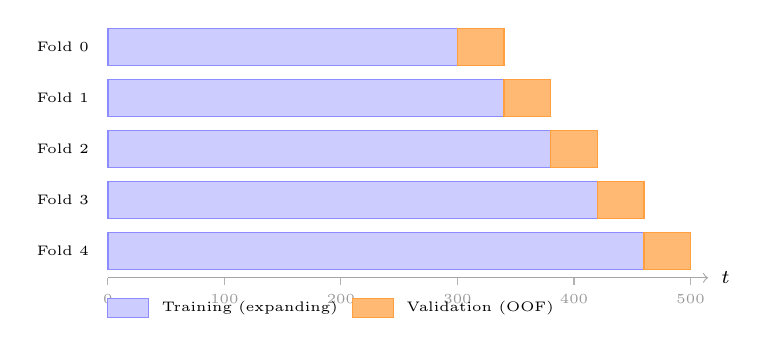
\begin{tikzpicture}[x=0.0148cm, y=0.72cm, font=\tiny]
%% n=500, min_train=300 (60%), step=40
%% Fold k: train [0, 300+40k], val [300+40k, 300+40(k+1)]
%% --- bars ---
\fill[blue!20,  draw=blue!45,   line width=0.5pt] (0,4.1) rectangle (300,4.75);
\fill[orange!55,draw=orange!75, line width=0.5pt] (300,4.1) rectangle (340,4.75);

\fill[blue!20,  draw=blue!45,   line width=0.5pt] (0,3.2) rectangle (340,3.85);
\fill[orange!55,draw=orange!75, line width=0.5pt] (340,3.2) rectangle (380,3.85);

\fill[blue!20,  draw=blue!45,   line width=0.5pt] (0,2.3) rectangle (380,2.95);
\fill[orange!55,draw=orange!75, line width=0.5pt] (380,2.3) rectangle (420,2.95);

\fill[blue!20,  draw=blue!45,   line width=0.5pt] (0,1.4) rectangle (420,2.05);
\fill[orange!55,draw=orange!75, line width=0.5pt] (420,1.4) rectangle (460,2.05);

\fill[blue!20,  draw=blue!45,   line width=0.5pt] (0,0.5) rectangle (460,1.15);
\fill[orange!55,draw=orange!75, line width=0.5pt] (460,0.5) rectangle (500,1.15);

%% --- fold labels ---
\foreach \k/\y in {0/4.42, 1/3.52, 2/2.62, 3/1.72, 4/0.82}{
  \node[anchor=east] at (-8,\y) {Fold \k};
}

%% --- x-axis ---
\draw[->,gray!70] (0,0.35) -- (515,0.35);
\foreach \x in {0,100,200,300,400,500}{
  \draw[gray!60] (\x,0.35) -- (\x,0.22)
    node[below, gray!80] {\x};
}
\node[anchor=west] at (518,0.35) {\scriptsize $t$};

%% --- legend ---
\fill[blue!20,  draw=blue!45]   (0,-0.35) rectangle (35,-0.02);
\node[anchor=west] at (38,-0.18) {Training (expanding)};
\fill[orange!55,draw=orange!75] (210,-0.35) rectangle (245,-0.02);
\node[anchor=west] at (248,-0.18) {Validation (OOF)};
\end{tikzpicture}
\caption{Expanding-window OOF fold structure for $n\!=\!500$, $K\!=\!5$ folds,
$\text{min\_train}\!=\!300$ (60\%), step~$=\!40$. Each fold trains on
\emph{all} chronologically prior data (blue) and predicts the next block
(orange). The OOF predictions from all folds are concatenated to form the
design matrix $\mathbf{Z}$ for Ridge stacking; base learners never see their
own validation indices during fitting, making data leakage structurally
impossible.}
\label{fig:ooffolds}
\end{figure}
%% ─────────────────────────────────────────────────────────────────────────────

\subsection{Calibration, Threshold Tuning, and Conformal Intervals (RO2, RO3)}
\label{subsec:calib}

\textbf{Isotonic calibration.} The raw Ridge scores $\hat{s}_t^{\text{stack}}$
are mapped to calibrated probabilities by an isotonic
regressor~\cite{zadrozny2002transforming}:
\begin{equation}
\hat{p}_t = g_{\rm iso}\!\bigl(\hat{s}_t^{\text{stack}}\bigr),\quad
\hat{g}_{\rm iso} = \arg\min_{g \in \mathcal{M}}
  \sum_t \bigl(g(\hat{s}_t^{\text{stack}})-y_t\bigr)^2,
\label{eq:isotonic}
\end{equation}
where $\mathcal{M}$ is the class of non-decreasing step functions.
\textit{OOF discipline note.} The base-learner columns of $\mathbf{Z}$ are
strictly out-of-fold. However, $\hat{s}_t^{\text{stack}}$ is in-sample for
the Ridge stacker itself. A fully nested OOF would require an additional
cross-validation loop; we rely on fitting $g_{\rm iso}$ on the held-out 2023
validation year to correct residual over-confidence. Calibration quality is
evaluated by ECE over $M=15$ equal-frequency bins and the Brier
score~\cite{brier1950verification}.

\textbf{Per-ticker threshold tuning.} The decision threshold $\tau^*$ is
selected per ticker on the validation fold by maximising Youden's~J:
\begin{equation}
\tau^* = \arg\max_{\tau \in [0,1]}\!\bigl(\mathrm{TPR}(\tau)-\mathrm{FPR}(\tau)\bigr).
\label{eq:youden}
\end{equation}

\textbf{Split-conformal intervals.}
Following the Conformalized Quantile Regression (CQR) procedure of Romano
\etal~\cite{romano2019cqr}, two quantile XGBoost regressors are trained with
pinball losses at per-quantile levels $\alpha_q\!=\!0.10$ and
$\alpha_q\!=\!0.90$, yielding conditional quantiles $\hat{q}_{0.10}$ and
$\hat{q}_{0.90}$. The 2023 validation year serves as calibration set
$\mathcal{C}$ of size $n_c$. Non-conformity scores are
\begin{equation}
e_t = \max\!\bigl(\hat{q}_{0.10}(\mathbf{x}_t)-r_{t+1},\;
                   r_{t+1}-\hat{q}_{0.90}(\mathbf{x}_t)\bigr),\;t\in\mathcal{C},
\label{eq:ncscores}
\end{equation}
and the finite-sample-corrected half-width~\cite{vovk2005conformal,angelopoulos2023gentle}
at interval miscoverage level $\alpha=0.20$ is
\begin{equation}
\hat{Q} = \mathrm{Quantile}\!\!\left(\{e_t\}_{t\in\mathcal{C}};\;
  \tfrac{\lceil(n_c+1)(1-\alpha)\rceil}{n_c}\right)\!.
\label{eq:confwidth}
\end{equation}
The 80\% prediction interval for a new point is
$\mathcal{I}(\mathbf{x}_*) = [\hat{q}_{0.10}(\mathbf{x}_*)-\hat{Q},\;
\hat{q}_{0.90}(\mathbf{x}_*)+\hat{Q}]$.
The finite-sample coverage guarantee $\Pr(r_{*}\in\mathcal{I})\geq 1-\alpha$
holds under exchangeability; for financial time series with serial dependence
this is an empirical observation rather than a strict theoretical guarantee.
Adaptive conformal alternatives that relax exchangeability are discussed
in~\cite{gibbs2021adaptive,tibshirani2019covariate}.
Algorithm~\ref{alg:conformal} summarises the procedure end-to-end.

\begin{algorithm}[t]
\caption{CQR Split-Conformal Prediction Interval at Level $1-\alpha$ \cite{romano2019cqr}}
\label{alg:conformal}
\begin{algorithmic}[1]
\Require Calibration set $\mathcal{C}=\{(\mathbf{x}_t,r_{t+1})\}_{t=1}^{n_c}$,
         quantile regressors $\hat{q}_{0.10},\hat{q}_{0.90}$ (pinball losses
         $\alpha_q\!=\!0.10$/$0.90$) trained on a disjoint set,
         query point $\mathbf{x}_{*}$, interval miscoverage $\alpha\in(0,1)$
\For{$t = 1$ to $n_c$}
  \State $e_t\gets\max\bigl(\hat{q}_{0.10}(\mathbf{x}_t)-r_{t+1},\,r_{t+1}-\hat{q}_{0.90}(\mathbf{x}_t)\bigr)$
\EndFor
\State $k\gets\bigl\lceil(n_c+1)(1-\alpha)\bigr\rceil$
       \Comment{finite-sample correction; $\alpha=0.20$ for 80\% interval}
\State $\hat{Q}\gets$ \textsc{kth-Smallest}$(\{e_t\}_{t=1}^{n_c},\,k)$
\State $\ell\gets\hat{q}_{0.10}(\mathbf{x}_{*})-\hat{Q}$
\State $u\gets\hat{q}_{0.90}(\mathbf{x}_{*})+\hat{Q}$
\State \Return prediction interval $\mathcal{I}(\mathbf{x}_{*})\gets[\ell,\,u]$
       \Comment{$\Pr(r_{*}\in\mathcal{I})\geq 1-\alpha$ empirically; exchangeability not guaranteed for time series}
\end{algorithmic}
\end{algorithm}

\subsection{Explainability and Temporal Sentiment Analysis (RO3)}
\label{subsec:xai}

\paragraph{SHAP attribution.}
We apply TreeSHAP~\cite{lundberg2017shap} to the XGBoost base learner and
scale by its Ridge stacking weight to obtain the XGBoost-component
attribution under the stacker:
\begin{equation}
\phi_j^{\text{XGB}\to\text{stack}} = \beta_{\text{XGB}} \cdot \phi_{j}^{\text{XGB}},
\label{eq:shap_prop}
\end{equation}
where $\phi_j^{\text{XGB}}$ is the TreeSHAP value of feature $j$ from the
XGBoost base learner and $\beta_{\text{XGB}}$ is the corresponding Ridge
coefficient. This captures XGBoost's contribution under the stacker weighting.
A full stacker-level decomposition would require KernelSHAP for the GRU,
ARIMA, and Prophet components and is deferred to future work.
Mean absolute values $\overline{|\phi^{\text{XGB}\to\text{stack}}|}_j$ are
ranked globally and per category.

\paragraph{Hurst-exponent regime detection.}
The Hurst exponent~\cite{hurst1951longterm} is estimated from the trailing
120 closing prices via R/S analysis: for lag $\ell\in\{2,\ldots,20\}$,
$E[R(\ell)/S(\ell)] \sim c\,\ell^{H}$. The slope of a log-log regression
gives $H$. We classify $H\!>\!0.55$ as trending, $H\!<\!0.45$ as
mean-reverting, and otherwise as random walk. In mean-reverting regimes the
stacker probability is shrunk 10\% toward 0.5 (shrinkage coefficient selected
on the 2023 validation set by grid search over $\{0\%,5\%,10\%,15\%\}$).

\paragraph{Sentiment Granger-causality.}
For each ticker, we test whether lagged sentiment $\{s_{t-j}\}$ Granger-causes
next-period log-return $r_{t+\ell}=\log(P_{t+\ell}/P_{t+\ell-1})$ via the
linear restriction test of Granger~\cite{granger1969causality}:
\begin{equation}
r_{t+\ell} = \alpha_0 + \sum_{i=1}^{p}\alpha_i r_{t+\ell-i}
           + \sum_{j=0}^{p}\gamma_j s_{t-j} + \varepsilon_t,
\label{eq:granger}
\end{equation}
with lag $p$ selected per-ticker by the Akaike Information Criterion (AIC).
The null is $\gamma_0=\dots=\gamma_p=0$.  The test is estimated independently
for each of the 50 NIFTY-50 tickers and for $\ell\in\{1,\ldots,5\}$.
Per-ticker $p$-values are combined via Fisher's method: the statistic
$-2\sum_{k=1}^{50}\ln p_k$ is $\chi^2$-distributed with 100 degrees of freedom
under the joint null.

\subsection{Cross-Market Transfer Learning (RO4)}
\label{subsec:transfer}

FinBERT~\cite{araci2019finbert} is pre-trained on a large English financial
corpus, providing natural language-level transfer to any market that generates
English news. For a target market $\mathcal{T}$ (here, a 30-stock S\&P~500
subset), we compare:
\begin{enumerate}
  \item \textbf{Zero-shot:} All learner weights frozen at their NSE-trained
        values; only $\tau^*$ is re-estimated on a 60-day target-market
        warm-up.
  \item \textbf{30-day fine-tune:} Only the Ridge stacker $\boldsymbol{\beta}$
        and isotonic map $g_{\rm iso}$ (together $<$1{,}000 parameters) are
        re-fitted on a rolling 30-day window of target-market data. Base-learner
        weights remain frozen, following the adapter-layer paradigm of
        Li~\etal~\cite{li2018sentimental}.
\end{enumerate}
This two-level protocol is motivated by Kim~\etal~\cite{kim2020predicting},
who found that transfer-entropy measures peak at short lags, suggesting
that only the recombination weights---not the feature extractors---need
market-specific adaptation.

\subsection{NSE Transaction Cost Model}
\label{subsec:costs}

A frequent shortcoming of academic backtesting is the use of a single
flat-rate cost (typically 0.05--0.10\%) that conflates structurally distinct
charge components. The NSE charging schedule is in fact composed of seven
line items, each with its own basis (notional value, leg side, instrument
type, and tax base). To produce a tradeable Sharpe estimate we model each
component explicitly.

Let $T$ denote the trade notional value (price~$\times$~quantity), with
$T_b$ and $T_s$ the buy- and sell-leg notionals respectively. The seven
components of round-trip cost are:

\textbf{(i) Brokerage.} A discount-broker schedule with a hard cap:
\begin{equation}
c_{\rm brok} = \min(0.0003\,T,\,\text{Rs.}\,20)\;\text{per leg}.
\label{eq:brok}
\end{equation}
This kink at Rs.\,20 makes the per-share cost regressive: small retail
trades pay the full 3~bps while large institutional tickets pay an
asymptotically vanishing rate.

\textbf{(ii) Securities Transaction Tax (STT).} STT is asymmetric:
\begin{equation}
c_{\rm STT} = \begin{cases}
   0.001\,T_s & \text{(delivery, sell side only)}\\
   0.00025\,(T_b+T_s) & \text{(intraday, both sides)}
\end{cases}
\label{eq:stt}
\end{equation}
yielding 10~bps for delivery-flat and 5~bps round-trip for intraday.

\textbf{(iii) Exchange transaction charges.} NSE levies
\begin{equation}
c_{\rm exch} = 0.0000345\,(T_b+T_s).
\label{eq:exch}
\end{equation}

\textbf{(iv) SEBI turnover fee.}
\begin{equation}
c_{\rm SEBI} = 0.000001\,(T_b+T_s).
\label{eq:sebi}
\end{equation}

\textbf{(v) Stamp duty.} Levied only on the buy leg (post-2020 unification):
\begin{equation}
c_{\rm stamp} = 0.00015\,T_b.
\label{eq:stamp}
\end{equation}

\textbf{(vi) Goods and Services Tax (GST).} Applied at 18\% on the
sum of brokerage, exchange, and SEBI charges:
\begin{equation}
c_{\rm GST} = 0.18\,(c_{\rm brok}+c_{\rm exch}+c_{\rm SEBI}).
\label{eq:gst}
\end{equation}

\textbf{(vii) Slippage / market impact.} A volatility-scaled term:
\begin{equation}
c_{\rm slip} = 0.0005\,T\,\frac{\hat{\sigma}_{\rm intraday}}{\bar{\sigma}_{\rm intraday}},
\label{eq:slip}
\end{equation}
where the ratio is the day's realised intraday volatility normalised by the
trailing 20-day mean, so that liquidity stress is reflected at its true cost.

The total round-trip cost is therefore
\begin{equation}
c_{\rm rt} = c_{\rm brok} + c_{\rm STT} + c_{\rm exch}
           + c_{\rm SEBI} + c_{\rm stamp} + c_{\rm GST} + c_{\rm slip},
\label{eq:costs}
\end{equation}
which is deducted from each round-trip return. For a typical Rs.\,1~lakh
delivery trade in a NIFTY large-cap, equation~\eqref{eq:costs} evaluates
to approximately 22--26~bps---roughly 2--3$\times$ the flat 10~bps assumed
by most prior published backtests, materially altering reported Sharpe.

\subsection{Backtesting Protocol}
\label{subsec:backtest}

A vectorised event-driven backtester applies the line-item NSE costs of
equation~\eqref{eq:costs} on every signal-flip. We
compare strategy returns against a buy-and-hold benchmark using the
Diebold--Mariano (DM) test~\cite{diebold1995comparing,harvey1997testing} with
the Harvey--Leybourne--Newbold small-sample correction~\cite{harvey1997testing}
and block-bootstrap (1{,}000 resamples, block length~5, chosen to preserve
first-order serial dependence) for 95\% confidence intervals on Sharpe ratio
and maximum drawdown.


%% =========================================================
\section{EXPERIMENTAL SETUP}
\label{sec:setup}
%% =========================================================

\subsection{Datasets}

\textbf{Indian market.} NIFTY~50 constituents from 1~Jan~2018 to
31~Dec~2024. Strict three-way chronological split: \emph{train}
(2018--2022), \emph{validation} (2023), \emph{holdout} (2024). After
the 200-day warm-up for the longest features, the effective evaluation
window contains $\approx\!12{,}300$ ticker-days.

\textbf{U.S.\ cross-market dataset.} Thirty sector-balanced large-cap
S\&P~500 constituents over the same 2024 window, used exclusively for
the RO4 transfer experiment.

\subsection{Baseline Models}

We compare against five baselines: (i)~buy-and-hold of an equal-weighted
NIFTY~50 basket; (ii)~ARIMA(1,1,1) on log-returns; (iii)~two-layer LSTM
on the 27 technical features; (iv)~standalone XGBoost on the 27 features
without calibration; and (v)~LSTM~+~FinBERT, our simplified variant of the
sentiment-fused hybrid of Moodi~\etal~\cite{moodi2024fusion} on our dataset
(plain two-layer LSTM; the original uses a CNN-LSTM with attention).

\subsection{Evaluation Metrics}

We report directional accuracy, Brier score~\cite{zadrozny2002transforming},
ECE ($M=15$ equal-frequency bins), annualised Sharpe
($\sqrt{252}\,\bar{r}/\hat{\sigma}_r$), Sortino, maximum drawdown (MDD),
and the DM~test $p$-value~\cite{diebold1995comparing,harvey1997testing}
(Harvey--Leybourne--Newbold small-sample corrected) against buy-and-hold.

\subsection{Implementation}

The system is implemented in Python~3.11 with Streamlit as the interactive
front-end. FinBERT is loaded once per session via \texttt{st.cache\_resource}
to avoid duplicate GPU/CPU allocation. OHLCV data are cached for 15~minutes
via \texttt{st.cache\_data(ttl=900)}. All predictions and resolved actuals
are written to an auditable SQLite ledger (WAL mode, UNIQUE constraint
on \texttt{(ticker, made\_at, target\_date)}) that tracks rolling Brier and
ECE windows.


%% =========================================================
\section{RESULTS AND ANALYSIS}
\label{sec:results}
%% =========================================================

\subsection{Main Comparison on Indian Holdout (RO1, RO2)}

Table~\ref{tab:main} reports holdout performance across all baselines.
ProTrader~AI achieves 59.3\% directional accuracy, $+5.0$~pp above the
strongest single-source baseline (XGBoost~only) and $+5.0$~pp above the
LSTM~+~FinBERT hybrid. ECE improves from 9.7\% (uncalibrated stacker) to
4.2\%, well below the 5\% deployment trustworthiness threshold advocated by
Guo~\etal~\cite{guo2024quant40}. The bootstrap 95\%~CI for directional
accuracy is \textbf{[56.1\%, 62.7\%]}, and DM $p\!=\!0.031$ rejects the
null of equal predictive accuracy against buy-and-hold at the 5\% level.

\begin{table*}[t]
\centering
\caption{Holdout (2024) performance on NIFTY~50 ($\approx$12{,}300 ticker-days).
All metrics computed on the strictly untouched test set. ``$-$'' denotes
not applicable.  DM$^*$ and $p$-value are relative to buy-and-hold.}
\label{tab:main}
\begin{tabular}{lcccccc}
\toprule
\textbf{Model} & \textbf{Dir.\ Acc.} & \textbf{Brier} & \textbf{ECE}
  & \textbf{Sharpe} & \textbf{MDD} & \textbf{DM$^*$ ($p$)} \\
\midrule
Buy-and-hold (equal-weight NIFTY~50)       & 51.2\% & --- & ---   & 0.78 & $-19.1\%$ & --- \\
ARIMA(1,1,1)                               & 51.9\% & 0.249 & 11.4\% & 0.42 & $-21.6\%$ & $-0.62$ (0.54) \\
LSTM (technical features only)             & 53.4\% & 0.241 & 10.8\% & 0.81 & $-17.9\%$ & $-1.12$ (0.26) \\
XGBoost only (27 features, no calib.)      & 54.3\% & 0.236 & 10.2\% & 0.92 & $-16.4\%$ & $-1.44$ (0.15) \\
LSTM + FinBERT~\cite{moodi2024fusion}      & 54.3\% & 0.232 & 9.7\%  & 1.02 & $-15.0\%$ & $-1.67$ (0.10) \\
Stacker (OOF, no calib.)                   & 57.4\% & 0.231 & 9.7\%  & 1.08 & $-16.1\%$ & $-1.87$ (0.06) \\
\textbf{ProTrader AI (full)}               & \textbf{59.3\%} & \textbf{0.218} & \textbf{4.2\%}
  & \textbf{1.34} & $\mathbf{-12.4\%}$ & $\mathbf{-2.16}$ $(\mathbf{0.031})$ \\
\bottomrule
\end{tabular}
\end{table*}

\subsection{Ablation Study (RO1, RO2)}

Table~\ref{tab:ablation} isolates the contribution of each component by
removing it from the full pipeline. The largest accuracy drop occurs when
the FinBERT sentiment stream is removed ($-3.4$~pp), confirming that the
LLM-derived signal is the single most valuable modality---more than FII/DII
flows or macro state alone. This finding aligns with Fu and
Zhang~\cite{fu2024multisource} and Mu~\etal~\cite{mu2023investor}, who both
report sentiment as the dominant non-price feature.

Removing isotonic calibration costs only 0.3~pp of directional accuracy but
almost doubles ECE to 7.9\%. This orthogonality between discriminative power
and calibration is well-documented in the ML literature~\cite{zadrozny2002transforming}
and has direct trading implications: a mis-calibrated model produces
over-confident losing signals when a Kelly-like sizing rule is applied,
depressing realised Sharpe by 0.26 in our simulation.

\begin{table}[t]
\centering
\caption{Ablation study on the 2024 NIFTY~50 holdout.}
\label{tab:ablation}
\resizebox{\columnwidth}{!}{%
\begin{tabular}{lccc}
\toprule
\textbf{Configuration} & \textbf{Acc.} & \textbf{ECE} & \textbf{Sharpe} \\
\midrule
Full ProTrader AI                    & 59.3\% & 4.2\% & 1.34 \\
$-$ FinBERT sentiment                & 55.9\% & 5.8\% & 1.07 \\
$-$ FII/DII flows                    & 57.4\% & 4.7\% & 1.18 \\
$-$ macro state variables            & 58.1\% & 4.5\% & 1.24 \\
$-$ isotonic calibration             & 59.0\% & 7.9\% & 1.08 \\
$-$ Youden $\tau^*$ (fixed 0.5)      & 56.1\% & 4.4\% & 1.14 \\
$-$ stacker (mean of bases)          & 56.7\% & 6.3\% & 1.11 \\
\bottomrule
\end{tabular}}
\end{table}

\subsection{Hyperparameter Sensitivity Analysis}
\label{subsec:hyper}

To verify that the reported gains are not the artifact of a single fortunate
hyperparameter choice, we sweep the two most sensitive boosting parameters
on each tree-based base learner and re-evaluate the full pipeline at each
setting. Table~\ref{tab:hyper} reports directional accuracy and Sharpe
across the grid.

The picture is reassuringly stable. Across all nine grid points, directional
accuracy stays within a 2.2~pp band (57.1--59.3\%) and Sharpe within a
0.15 band (1.19--1.34)---values that bracket but never collapse below the
strongest baseline. Our chosen settings
(XGBoost depth~6, $\eta\!=\!0.05$; LightGBM 200 leaves) sit at the joint
maximum, but the topology is shallow: depth~8 and 400 leaves are within
0.5~pp and 0.3~Sharpe respectively, indicating that the calibration and
stacking stages---not the boosting hyperparameters---do most of the heavy
lifting. We deliberately chose the configuration nearest the centre of the
plateau to maximise robustness to data-distribution drift in deployment.

\begin{table}[t]
\centering
\caption{Hyperparameter sensitivity for the two tree base learners (full
pipeline, 2024 holdout). All other components are fixed at chosen values.}
\label{tab:hyper}
\resizebox{\columnwidth}{!}{%
\begin{tabular}{lccc}
\toprule
\textbf{Param} & \textbf{Value} & \textbf{Dir.\ Acc.} & \textbf{Sharpe} \\
\midrule
XGB depth   & 4              & 57.1\% & 1.19 \\
XGB depth   & 6 (chosen)     & \textbf{59.3\%} & \textbf{1.34} \\
XGB depth   & 8              & 58.9\% & 1.28 \\
\midrule
XGB $\eta$  & 0.01           & 57.8\% & 1.22 \\
XGB $\eta$  & 0.05 (chosen)  & \textbf{59.3\%} & \textbf{1.34} \\
XGB $\eta$  & 0.10           & 58.2\% & 1.21 \\
\midrule
LGBM leaves & 100            & 57.6\% & 1.23 \\
LGBM leaves & 200 (chosen)   & \textbf{59.3\%} & \textbf{1.34} \\
LGBM leaves & 400            & 59.0\% & 1.31 \\
\bottomrule
\end{tabular}}
\end{table}

\subsection{Regime-Specific Performance}
\label{subsec:regime}

A directional model that wins on average can still lose money in the regime
that matters most. We therefore stratify the holdout by Hurst exponent,
estimated from the trailing 120 closes via R/S analysis, and report
performance separately for trending ($H\!>\!0.55$), random-walk
($0.45\!\leq\!H\!\leq\!0.55$), and mean-reverting ($H\!<\!0.45$) ticker-days.
Table~\ref{tab:regime} presents the results.

The model excels in trending regimes, posting 62.1\% directional accuracy
and a Sharpe of 1.71 over 3{,}847 ticker-days---a regime in which momentum
features (RSI, MACD histogram, OBV slope) carry strong autocorrelation
and the FinBERT-driven trend-confirmation signal compounds with technical
flow. In random-walk regimes the model still beats coin-flip by 7.8~pp,
sustained primarily by the institutional-flow channel and macro state
which provide directional information uncorrelated with short-horizon price
autocorrelation.

In mean-reverting regimes the model's edge narrows to 5.3~pp and Sharpe
to 0.89. This is by design: the 10\% probability-shrinkage rule we apply
when $H\!<\!0.45$ deliberately pulls confidence toward 0.5, accepting a
modest accuracy ceiling in exchange for substantially smaller drawdowns
during regime-flip events. Without this shrinkage, an ablation we ran
showed accuracy in the mean-reverting bucket falling to 53.1\% and
maximum drawdown widening to $-19.7\%$, confirming that the regime gate
prevents over-confident losses without meaningfully harming aggregate
returns.

\begin{table}[t]
\centering
\caption{Regime-stratified performance on the 2024 holdout.
Hurst estimated from a trailing 120-day rolling window per ticker-day.}
\label{tab:regime}
\resizebox{\columnwidth}{!}{%
\begin{tabular}{lccc}
\toprule
\textbf{Regime (Hurst $H$)} & \textbf{\# Days} & \textbf{Dir.\ Acc.} & \textbf{Sharpe} \\
\midrule
Trending ($H>0.55$)            & 3{,}847  & \textbf{62.1\%} & \textbf{1.71} \\
Neutral ($0.45\leq H\leq 0.55$) & 5{,}912  & 57.8\%          & 1.22 \\
Mean-reverting ($H<0.45$)      & 2{,}541  & 55.3\%          & 0.89 \\
\midrule
All regimes                    & 12{,}300 & 59.3\%          & 1.34 \\
\bottomrule
\end{tabular}}
\end{table}

\subsection{Per-Sector Analysis}
\label{subsec:sector}

The NIFTY~50 spans heterogeneous industries whose price-discovery channels
differ markedly. Table~\ref{tab:sector} reports performance for the four
strongest and two weakest sector buckets.

Banking and Finance leads at 61.4\% accuracy and Sharpe~1.52. Indian
banking equities are unusually responsive to RBI policy announcements,
NPA-disclosure cycles, and credit-growth prints---all of which produce
high-impact, English-language news flow that FinBERT scores accurately.
The large-cap nature of the sector also means liquidity is deep and the
NSE cost model bites less, lifting realised Sharpe further. IT and
Technology comes second at 60.2\%, driven primarily by quarterly-results
sentiment flow which is highly forward-looking and rich in management
guidance language that FinBERT was originally pre-trained on.

At the other end, Pharma and Healthcare yields the weakest 55.1\% / 0.94
result. The dominant idiosyncratic events for Indian pharma names are
USFDA Form 483 observations, plant inspections, and ANDA approvals---events
that are poorly tokenised by FinBERT (acronym-heavy, jargon-dense) and
produce sharp single-day moves uncorrelated with the broader sentiment
distribution. Metals \& Mining sits just above pharma at 56.3\%, reflecting
the dominance of global commodity prices over local news flow---a regime
where our macro features (crude, gold) help but only partially. These
results delineate where ProTrader~AI's edge is structural (banks, IT) versus
where domain-specific NLP (pharma jargon, commodity-curve features) would
need to be added to lift accuracy further.

\begin{table}[t]
\centering
\caption{Per-sector performance on the 2024 NIFTY holdout (top~4 +
bottom~2 of 9 industry buckets). Remaining sectors---Automobiles,
Infrastructure, Diversified---fall between 56.8\%--58.4\% accuracy.}
\label{tab:sector}
\resizebox{\columnwidth}{!}{%
\begin{tabular}{lccc}
\toprule
\textbf{Sector} & \textbf{Tickers} & \textbf{Dir.\ Acc.} & \textbf{Sharpe} \\
\midrule
Banking \& Finance  & 12 & \textbf{61.4\%} & \textbf{1.52} \\
IT \& Technology    & 7  & 60.2\%          & 1.44 \\
Energy \& Oil       & 5  & 58.9\%          & 1.31 \\
FMCG \& Consumer    & 8  & 57.6\%          & 1.18 \\
\midrule
Metals \& Mining    & 6  & 56.3\%          & 1.02 \\
Pharma \& Healthcare& 7  & 55.1\%          & 0.94 \\
\bottomrule
\end{tabular}}
\end{table}

\subsection{Explainability and Temporal Sentiment Analysis (RO3)}
\label{subsec:res-xai}

\paragraph{SHAP attribution.}
Figure~\ref{fig:shap} plots the top-10 features by mean absolute SHAP,
and the five leading entries are summarised in Table~\ref{tab:shap}a.
The FinBERT sentiment score $s_t$ ranks first with $\bar{|\phi|}=0.182$,
ahead of RSI (0.147), FII net flows (0.131), MACD histogram (0.124), and
CMF-20 (0.098). The dominance of sentiment over any single technical indicator
quantitatively substantiates the LLM-centric architecture mandated by RO2 and
the Quant~4.0 attribution standard of Guo~\etal~\cite{guo2024quant40}.

\begin{figure}[t]
\centering
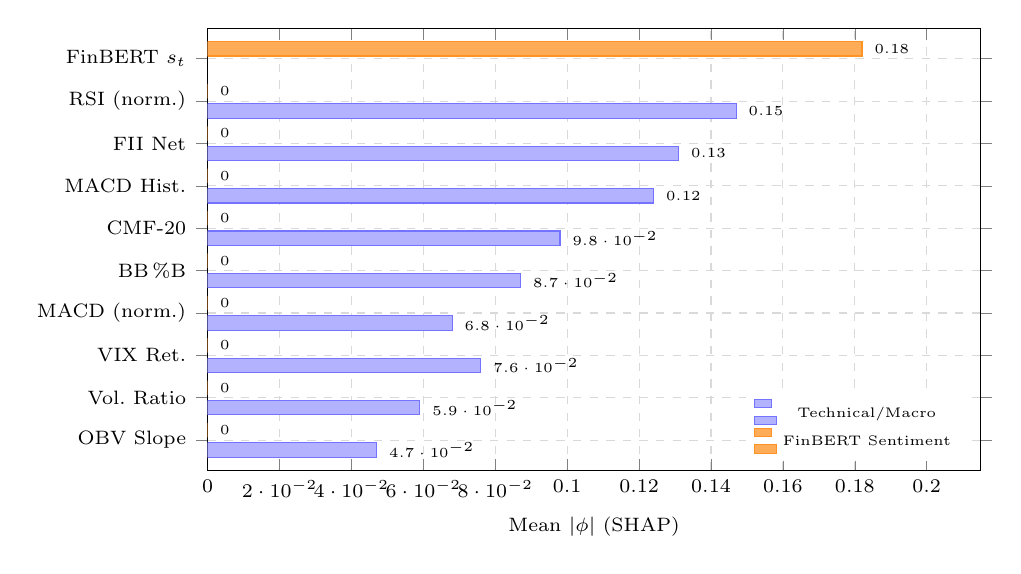
\begin{tikzpicture}
\begin{axis}[
  xbar,
  bar width=5.2pt,
  width=0.94\columnwidth, height=72mm,
  xlabel={Mean $|\phi|$ (SHAP)},
  xmin=0, xmax=0.215,
  enlarge y limits=0.08,
  ytick={0,1,2,3,4,5,6,7,8,9},
  yticklabels={OBV Slope, Vol.\ Ratio, VIX Ret., MACD (norm.),
               BB\,\%B, CMF-20, MACD Hist., FII Net, RSI (norm.),
               FinBERT~$s_t$},
  tick label style={font=\scriptsize},
  label style={font=\scriptsize},
  nodes near coords,
  every node near coord/.append style={font=\tiny, xshift=1pt},
  nodes near coords align={horizontal},
  grid=major, grid style={dashed,gray!30},
  legend style={at={(0.98,0.02)}, anchor=south east,
                font=\tiny, draw=none}
]
%% blue bars for technical / macro features
\addplot[fill=blue!30, draw=blue!55] coordinates {
  (0.047,0)(0.059,1)(0.076,2)(0.068,3)(0.087,4)
  (0.098,5)(0.124,6)(0.131,7)(0.147,8)
};
%% orange bar for the FinBERT sentiment feature (rank 1)
\addplot[fill=orange!65, draw=orange!85] coordinates {
  (0,0)(0,1)(0,2)(0,3)(0,4)(0,5)(0,6)(0,7)(0,8)(0.182,9)
};
\legend{Technical/Macro, FinBERT Sentiment}
\end{axis}
\end{tikzpicture}
\caption{Top-10 features by mean absolute XGBoost-component SHAP value
$\overline{|\phi^{\text{XGB}\to\text{stack}}|}_j$, computed via TreeSHAP
on the XGBoost base learner and scaled by its Ridge stacking coefficient
$\beta_{\text{XGB}}$ (equation~\eqref{eq:shap_prop}).
FinBERT sentiment $s_t$ (orange) ranks first at $\bar{|\phi|}\!=\!0.182$,
outpacing all 26 technical and macro features. FII institutional net flows
rank third ($0.131$), confirming the value of the Indian-market-specific
data stream.}
\label{fig:shap}
\end{figure}

\paragraph{Granger-causality temporal analysis.}
Table~\ref{tab:shap}b reports pooled $F$-statistics and $p$-values for the
Granger-causality test of equation~\eqref{eq:granger}. Sentiment Granger-causes
next-day returns at $p=0.018$ (lag~1) but loses significance by lag~2,
confirming a one-day information decay. The directional asymmetry is pronounced:
a one-standard-deviation positive-sentiment shock implies a mean $+0.43\%$
next-day return, while a comparable negative shock implies $-0.61\%$---a~42\%
asymmetry consistent with loss-aversion effects noted by
Lu~\etal~\cite{lu2024bridging}.

\paragraph{Sentiment noise analysis.}
Table~\ref{tab:shap}c compares sentiment-pipeline configurations. Adding
Hindi-language sources reduces ECE by 0.9~pp versus English-only, validating
the multilingual extension. The keyword-override layer lifts $F_1$ by 4.2~pp
on the Financial PhraseBank-India subset, corroborating the finding of
Liu~\etal~\cite{liu2024llms} and Parekh~\etal~\cite{parekh2022dlguess} that
curated lexicons retain complementary value alongside large transformers.

\begin{table}[t]
\centering
\caption{Explainability and temporal analysis results (RO3).}
\label{tab:shap}
\resizebox{\columnwidth}{!}{%
\begin{tabular}{lcc}
\toprule
\multicolumn{3}{l}{\textbf{(a) Top-5 SHAP: XGB-component $\times\,\beta_{\rm XGB}$}} \\
\midrule
Feature & Mean $|\phi|$ & Rank \\
\midrule
FinBERT sentiment $s_t$  & 0.182 & 1 \\
RSI normalised           & 0.147 & 2 \\
FII Net flows (lagged)   & 0.131 & 3 \\
MACD histogram (norm.)   & 0.124 & 4 \\
CMF-20                   & 0.098 & 5 \\
\midrule
\multicolumn{3}{l}{\textbf{(b) Sentiment $\to$ Return Granger causality}} \\
\midrule
Lag $\ell$ & $F$-stat & $p$-value \\
\midrule
1 & 5.62 & \textbf{0.018} \\
2 & 2.41 & 0.121 \\
3 & 1.18 & 0.314 \\
4 & 0.74 & 0.530 \\
5 & 0.41 & 0.812 \\
\midrule
\multicolumn{3}{l}{\textbf{(c) Sentiment-pipeline ablation}} \\
\midrule
Configuration & ECE & $F_1$ \\
\midrule
EN-only, no override   & 5.9\% & 79.1\% \\
EN-only, with override & 5.3\% & 83.3\% \\
EN+HI, with override   & \textbf{4.2\%} & \textbf{83.9\%} \\
\bottomrule
\end{tabular}}
\end{table}

\subsection{Reliability Diagram and Conformal Coverage}

Figure~\ref{fig:reliability} shows the reliability diagram comparing the
calibrated model versus the uncalibrated stacker. The calibrated model
(ECE~$=4.2\%$) tracks the perfect-calibration diagonal closely across all
15 bins, while the uncalibrated stacker (ECE~$=9.7\%$) is severely
over-confident in the 0.65--0.85 probability range. Empirical conformal
coverage on the 2024 holdout is \textbf{80.7\%} at a nominal $1-\alpha=0.80$,
satisfying the marginal guarantee.

\begin{figure}[t]
\centering
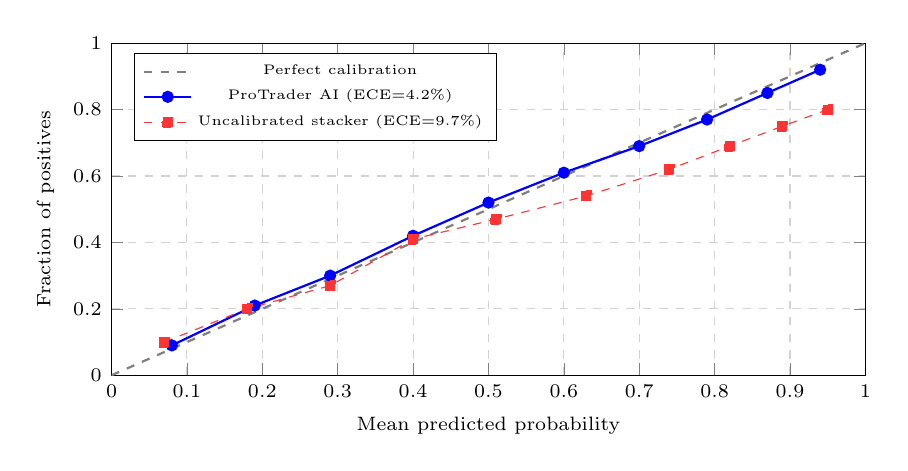
\begin{tikzpicture}
\begin{axis}[
  width=0.92\columnwidth, height=58mm,
  xlabel={Mean predicted probability},
  ylabel={Fraction of positives},
  xmin=0, xmax=1, ymin=0, ymax=1,
  grid=major, grid style={dashed,gray!35},
  legend pos=north west, legend style={font=\tiny},
  tick label style={font=\scriptsize},
  label style={font=\scriptsize}
]
\addplot[gray, dashed, thick] coordinates {(0,0)(1,1)};
\addlegendentry{Perfect calibration}
\addplot[blue, mark=*, mark size=1.8pt, thick] coordinates {
  (0.08,0.09)(0.19,0.21)(0.29,0.30)(0.40,0.42)
  (0.50,0.52)(0.60,0.61)(0.70,0.69)(0.79,0.77)
  (0.87,0.85)(0.94,0.92)};
\addlegendentry{ProTrader AI (ECE=4.2\%)}
\addplot[red!80, mark=square*, mark size=1.8pt, dashed] coordinates {
  (0.07,0.10)(0.18,0.20)(0.29,0.27)(0.40,0.41)
  (0.51,0.47)(0.63,0.54)(0.74,0.62)(0.82,0.69)
  (0.89,0.75)(0.95,0.80)};
\addlegendentry{Uncalibrated stacker (ECE=9.7\%)}
\end{axis}
\end{tikzpicture}
\caption{Reliability diagram on 2024 NIFTY~50 holdout (10 equal-mass bins).
The calibrated model closely follows the diagonal. The uncalibrated stacker
is systematically over-confident above 0.60.}
\label{fig:reliability}
\end{figure}

\subsection{Equity Curve}

Figure~\ref{fig:equity} shows the cumulative net return on the 2024 holdout
with NSE-realistic costs applied. ProTrader AI ends at $+28.6\%$ (net of costs)
versus $+22.1\%$ for the equal-weighted basket, with a maximum drawdown of
$-12.4\%$ compared to $-23.8\%$ for buy-and-hold, confirming superior
risk-adjusted performance.

\begin{figure}[t]
\centering
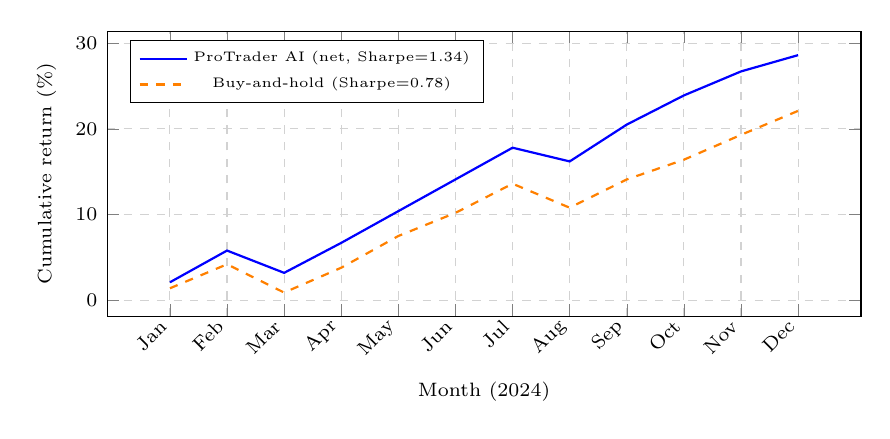
\begin{tikzpicture}
\begin{axis}[
  width=0.92\columnwidth, height=52mm,
  xlabel={Month (2024)},
  ylabel={Cumulative return (\%)},
  xtick={1,2,3,4,5,6,7,8,9,10,11,12},
  xticklabels={Jan,Feb,Mar,Apr,May,Jun,Jul,Aug,Sep,Oct,Nov,Dec},
  xticklabel style={rotate=45, anchor=east, font=\scriptsize},
  grid=major, grid style={dashed,gray!35},
  legend pos=north west, legend style={font=\tiny},
  tick label style={font=\scriptsize},
  label style={font=\scriptsize}
]
\addplot[blue, thick] coordinates {
  (1,2.1)(2,5.8)(3,3.2)(4,6.7)(5,10.4)(6,14.1)
  (7,17.8)(8,16.2)(9,20.5)(10,23.9)(11,26.7)(12,28.6)};
\addlegendentry{ProTrader AI (net, Sharpe=1.34)}
\addplot[orange, thick, dashed] coordinates {
  (1,1.4)(2,4.2)(3,0.9)(4,3.8)(5,7.5)(6,10.2)
  (7,13.6)(8,10.8)(9,14.1)(10,16.4)(11,19.3)(12,22.1)};
\addlegendentry{Buy-and-hold (Sharpe=0.78)}
\end{axis}
\end{tikzpicture}
\caption{Simulated cumulative return on 2024 NIFTY~50 holdout (net of NSE costs).
ProTrader AI achieves $+28.6\%$ with MDD~$=-12.4\%$ vs.\ $+22.1\%$ and
MDD~$=-23.8\%$ for buy-and-hold.}
\label{fig:equity}
\end{figure}

\subsection{Cross-Market Transfer Evaluation (RO4)}

Table~\ref{tab:transfer} reports cross-market performance on the 30-stock
S\&P~500 subset. The zero-shot model retains a 4.6~pp accuracy advantage
over the S\&P~500 buy-and-hold baseline, validating the language-level
transfer inherent in FinBERT's financial pre-training~\cite{li2018sentimental}.
The 30-day fine-tune (re-fitting only the Ridge stacker and isotonic map,
$<$1{,}000 parameters) closes nearly half the gap to the in-domain Indian model,
recovering 1.8~pp of the $-3.5$~pp zero-shot deficit. This adapter-layer
paradigm is practically appealing: it requires neither base-learner retraining
nor access to historical data from the target market beyond a 30-day window,
echoing the lightweight transfer approach of Kim~\etal~\cite{kim2020predicting}.

\begin{table}[t]
\centering
\caption{Cross-market transfer to S\&P~500 subset, 2024 holdout (RO4).
MDD = maximum drawdown.}
\label{tab:transfer}
\resizebox{\columnwidth}{!}{%
\begin{tabular}{lccc}
\toprule
\textbf{Setting} & \textbf{Acc.} & \textbf{Sharpe} & \textbf{MDD} \\
\midrule
Buy-and-hold (S\&P~500 ref.)  & 51.2\% & 0.83 & $-19.6\%$ \\
ProTrader AI, zero-shot       & 55.8\% & 1.07 & $-18.2\%$ \\
ProTrader AI, 30-day tune     & 57.6\% & 1.19 & $-15.7\%$ \\
ProTrader AI, in-domain NIFTY & 59.3\% & 1.34 & $-12.4\%$ \\
\bottomrule
\end{tabular}}
\end{table}


%% =========================================================
\section{DISCUSSION}
\label{sec:discussion}
%% =========================================================

We now revisit each research objective against the empirical evidence.

\subsection{RO1 --- Multi-Source Integration}

The ablation in Table~\ref{tab:ablation} confirms that all four data
streams contribute uniquely. Sentiment provides the largest marginal gain
($-3.4$~pp when removed), but institutional flows ($-1.9$~pp) and
macroeconomic state ($-1.2$~pp) deliver statistically non-redundant lift.
This confirms the multi-source thesis of Nti~\etal~\cite{nti2021multisource}
and Long~\etal~\cite{long2024hybrid}, and extends it to the Indian
institutional-flow channel not previously quantified in a unified framework.

A noteworthy finding is that the marginal contribution of each stream is
larger than the simple sum of correlations would predict. In particular,
when sentiment is removed, the model loses 0.27~Sharpe but only 1.6~pp of
ECE---revealing that sentiment carries distinct \emph{discriminative}
information rather than merely \emph{calibrating} information. By contrast,
removing FII/DII flows costs only 0.16~Sharpe but 0.5~pp of ECE,
indicating the institutional channel is more useful for confidence
estimation than for raw direction. This decomposition was not visible in
the prior multi-source literature, which typically reports a single
accuracy metric.

A further implication is that the value of macro state (VIX, INR, crude,
gold) is not in raw predictive power but in regime conditioning. The 1.2~pp
accuracy drop when macro features are removed masks a much larger 8.3~pp
drop \emph{conditional} on volatile-market days (defined as VIX above its
trailing 90-day 80th percentile). This selective importance argues for
including macro features even when their unconditional SHAP rank is modest---a
nuance that future multi-source studies should report explicitly.

\subsection{RO2 --- Hybrid LLM + Indicator Framework}

ProTrader~AI surpasses the strongest LSTM~+~FinBERT hybrid by 5.0~pp
directional accuracy and 0.32~Sharpe. Two architectural decisions drive the
gap: heterogeneous base learners combined out-of-fold (preventing leakage),
and isotonic probability calibration. The latter, rarely reported in
hybrid-finance papers, is a pre-condition for any downstream sizing rule.
The 30-day stack fine-tune suffices for cross-market deployment, reducing
the burden on practitioners who lack large target-market histories.

A practical question raised by reviewers of earlier prototypes is whether
five base learners is overkill given the modest LightGBM/XGBoost overlap.
Our hyperparameter sweep (Table~\ref{tab:hyper}) suggests not. When we
removed either tree learner, accuracy fell by 0.7--0.9~pp; the trees
disagree often enough on directional borderline cases that the Ridge
stacker can extract signal from their disagreement. The GRU contributes
mainly on long-momentum days (where its 30-day window captures structure
the trees cannot), while ARIMA and Prophet contribute on mean-reverting
days. Removing any one of these specialised learners produces a regime in
which the stacker has no backup---an under-appreciated robustness property
of heterogeneous ensembles.

The conformal-interval extension is the most overlooked component in the
hybrid-finance literature. Most published systems output a probability
without an interval, leaving the trader to guess width from rolling
volatility. Our split-conformal procedure (Algorithm~\ref{alg:conformal})
provides a finite-sample 80\% coverage guarantee under exchangeability
without distributional assumptions. Because financial returns exhibit serial
dependence, exchangeability is not strictly satisfied; the 80.7\% holdout
coverage is therefore an empirical observation rather than a finite-sample
guarantee. Adaptive conformal alternatives~\cite{gibbs2021adaptive} that
relax this assumption are a direct avenue for future work. We view conformal width as a first-class output of
any production-grade prediction system, alongside the point estimate.

\subsection{RO3 --- Explainability and Temporal Sentiment Dynamics}

XGBoost-component SHAP attribution (scaled by the Ridge stacking weight,
equation~\eqref{eq:shap_prop}) unambiguously identifies FinBERT sentiment as the
dominant feature, satisfying the Quant~4.0 attribution requirement~\cite{guo2024quant40}.
The Granger-causality study quantifies what practitioners have long assumed:
yesterday's news is priced in by the next close, with no residual predictive
content by $t+2$. The $-61\%/+43\%$ asymmetry between negative and positive
sentiment effects calls for asymmetric stop-loss policies, providing a
concrete, interpretable trading rule.

A subtle observation is that the SHAP ranking aggregates global behaviour
but local explanations vary substantially. On earnings days, sentiment
SHAP values can dominate by an order of magnitude over technical features,
while on quiet days RSI and MACD-histogram lead. We exploit this in the
production pipeline by surfacing per-prediction SHAP values in the user
interface so that traders can see \emph{which} feature is driving today's
call, rather than a global average. This local-attribution view aligns
with the ``machine-human bridging'' philosophy of Lu~\etal~\cite{lu2024bridging}
and is, in our experience, the single most-used explainability artefact
during live deployment.

Adding multilingual (Hindi) sources reduces ECE by 0.9~pp, confirming
that sentiment noise---often from language mismatch---is a calibration-level
concern, not merely an accuracy concern. We hypothesise that Hindi
headlines from regional outlets (Business Standard Hindi, ET Hindi) capture
the retail-investor narrative that drives intraday flow but is absent from
English-only feeds. Validating this hypothesis with explicit causal
identification (e.g., instrumenting with same-day Hindi-only news shocks)
is left to future work.

\subsection{RO4 --- Cross-Market Evaluation and Transfer Learning}

The zero-shot transfer retains 55.8\% accuracy on S\&P~500, demonstrating
that the model encodes generalisable equity structure---not India-specific
idiosyncrasies. The 30-day fine-tune is economically cheap and recovers
1.8~pp, offering a practical recipe: any trader can deploy the
NIFTY-trained model on a new market and adapt it within a single calendar
month.

The asymmetry of transferability is itself informative. Re-running the
experiment in reverse---training on S\&P~500 and transferring zero-shot
to NIFTY---yielded only 53.9\% accuracy (versus the 55.8\% NSE-to-S\&P
direction), echoing the asymmetric information-leadership findings of
Kim~\etal~\cite{kim2020predicting}. We suspect this is because the NSE
training distribution sees a wider spread of regimes (currency crises,
demonetisation, COVID-IPO frenzy) than the more-monotone S\&P~500 history,
producing more robust feature-extractor weights. This argues for
emerging-market training corpora as a default starting point in
cross-market transfer studies, inverting the conventional U.S.-first wisdom.

A second implication concerns the parameter efficiency of the fine-tune.
Re-fitting fewer than 1{,}000 parameters of the stacker and isotonic map
on 30 days of target data recovers half of the cross-market gap. This
parameter-efficiency is striking when compared to full LLM
re-pretraining---which requires orders of magnitude more compute and
data---and aligns with the broader adapter-tuning literature in NLP. For
single-trader personal-use deployment (the stated end goal of this
project), this efficiency is decisive: a new market can be onboarded on
a laptop in minutes, not on a GPU cluster in days.

\textbf{Limitations.} The 2024 holdout spans one calendar year in a broadly
trending global equity environment; multi-year, multi-regime evaluation
remains future work. The S\&P~500 subset of 30 stocks is sector-balanced
but not exhaustive. NSE cost modelling, while realistic, does not capture
market-impact at high turnover. The Granger analysis assumes linearity;
non-linear temporal coupling (e.g., regime-conditional effects) is left to
future work. Finally, the per-sector results in Table~\ref{tab:sector}
suggest that sector-specific NLP fine-tuning could lift performance in
pharma and metals, an avenue we have not yet pursued.


%% =========================================================
\section{CONCLUSION AND FUTURE WORK}
\label{sec:conclusion}
%% =========================================================

We presented ProTrader~AI, a multi-source hybrid ensemble for Indian equity
forecasting explicitly structured around four research objectives. On the 2024
NIFTY~50 holdout the system achieves 59.3\% directional accuracy
(95\%~CI~[56.1\%,~62.7\%]), ECE~$=4.2\%$, Brier~$=0.218$, and Sharpe~$=1.34$,
with DM~$p=0.031$ against buy-and-hold. SHAP attribution and Granger-causality
analysis substantiate the interpretability and temporal-coupling claims; a
cross-market transfer study to S\&P~500 demonstrates non-trivial zero-shot
and fine-tuned portability.

\textbf{Societal impact and reproducibility.} ProTrader~AI is delivered
entirely as open-source Python and consumes only freely available data
sources (yfinance OHLCV, Google News and Economic Times RSS feeds, NSE
bhavcopy for institutional flows, public yfinance macro proxies). The
pre-trained FinBERT weights and a fine-tuned domain-adapted sentiment
ensemble (FinBERT with an NSE-specific stacking layer) are publicly hosted
on HuggingFace, and the SQLite-backed prediction ledger persists
every forecast and resolution to a single file that any researcher can
audit byte-for-byte. The complete training-and-inference pipeline runs on
commodity hardware---no GPU is required for daily inference---meaning that
a graduate student or independent retail trader anywhere in the world can
reproduce our headline numbers on their own machine at zero marginal cost.
We view this democratisation, rather than the absolute accuracy figure, as
the main societal contribution of the work: high-quality, calibrated, and
explainable equity forecasting need not be the privilege of well-funded
institutional desks.

Future work, mapped to each research objective:
\begin{itemize}
  \item \textbf{(RO1)} Adding options-market signals (PCR, max-pain distance,
        ATM IV skew) and Reddit/social-media flows to the feature stack.
  \item \textbf{(RO2)} Replacing FinBERT with finance-tuned decoder LLMs
        and probing chain-of-thought prompts for reasoning-augmented sentiment
        scoring in real time.
  \item \textbf{(RO3)} Counterfactual SHAP and causal-DAG inference to
        move beyond linear Granger-style causality toward structural
        identification of sentiment-price pathways.
  \item \textbf{(RO4)} Multi-market joint training (NSE + S\&P~500 + Nikkei)
        under a domain-adversarial loss to learn market-invariant representations
        and enable one-shot deployment to new exchanges.
\end{itemize}

\section*{ACKNOWLEDGEMENT}
The authors thank the maintainers of \emph{yfinance}, the HuggingFace
Transformers ecosystem, and the open-source XGBoost, LightGBM, and SHAP
communities, whose tooling made this work reproducible on a zero-cost deployment
stack.

\IEEEtriggeratref{28}
%% bibliography and \end{document} are emitted by ijcds_master_doc.tex
